% ============================================================================
%  COMPILE WITH XeLaTeX  (twice, so the point total resolves)
%  Overleaf: Menu -> Compiler -> XeLaTeX
%  Requires: bnhandout.sty and fonts/Kalpurush.ttf in the project
% ============================================================================
\documentclass[11pt]{article}
\usepackage{bnhandout}          % add [nosol] for a student edition

\hauthor[https://jugantordey.github.io]{Jugantor Dey}
\hseries{Mathematics for the Physics Olympiad}

\begin{document}

\handouttitle{Chapter 18 : Complex Numbers}

\noindent
শুরু করার আগে ১৫ নম্বর অধ্যায়ের Taylor সিরিজের অনুচ্ছেদটি, ১৩ নম্বর
অধ্যায়ের যোগ সূত্র ও De Moivre-জাতীয় হিসাব, এবং ১০ নম্বর অধ্যায়ের
$\cosh$ ও $\sinh$ ঝালিয়ে নাও। ৩ নম্বর অধ্যায়ের দ্বিঘাত সমীকরণের সূত্রটিও
প্রথম অনুচ্ছেদেই লাগবে।

৩ নম্বর অধ্যায়ে দ্বিঘাত সমীকরণের সূত্র বের করার সময় একটি ক্ষেত্র খোলা রেখে
আসা হয়েছিল: নিশ্চায়ক $D < 0$ হলে বর্গমূলের ভেতরে ঋণাত্মক সংখ্যা পড়ে, আর
বাস্তব সমাধান থাকে না। তখন বলা হয়েছিল, ওই ক্ষেত্রটি এই অধ্যায়ে ফিরে আসবে।
এসেছে।

তবে এই অধ্যায়ের আসল গল্প অন্য জায়গায়। $i$-কে গণিতে ঢোকানো হয়েছিল কেবল
বীজগণিতের একটি ফাঁক বোজাতে, নিতান্ত হিসাবের সুবিধার জন্য। তারপর দেখা গেল সে
আসলে একটি জ্যামিতিক কাজ করে: সমতলে ঘূর্ণন। আর সেই আবিষ্কারের পর থেকে
পদার্থবিজ্ঞানে দোলন ও তরঙ্গ নিয়ে যত হিসাব হয়, তার প্রায় সবই জটিল সংখ্যায়
লেখা হয়, কারণ তাতে ত্রিকোণমিতির জঙ্গল সরে গিয়ে সরল গুণ-ভাগ থাকে।

একটি কথা আগেই বলে রাখি। চতুর্থ অনুচ্ছেদে Euler-এর সূত্র বের করা হবে Taylor
সিরিজ থেকে, এবং সেটিই এই অধ্যায়কে ১৫ নম্বরের পরে বসানোর কারণ। অনেক বইয়ে
$e^{i\theta} = \cos\theta + i\sin\theta$ কে সংজ্ঞা বলে চালিয়ে দেওয়া হয়; তখন
সূত্রটি প্রমাণ করার কিছু থাকে না, আর কেন এটি সত্য সেই প্রশ্নটাও হারিয়ে যায়।
এই অধ্যায়ে মোট \totalpoints\ পয়েন্ট আছে।

\section{কেন জটিল সংখ্যা দরকার}

$x^{2} + 1 = 0$ সমীকরণটির কোনো বাস্তব সমাধান নেই, কারণ বাস্তব সংখ্যার বর্গ
কখনো ঋণাত্মক হয় না (৯ নম্বর অধ্যায়ের সাত নম্বর নিয়ম)। কিন্তু সমাধান নেই
বলে থেমে না গিয়ে গণিতে বারবার যা করা হয়েছে, এখানেও তাই করা হলো: সংখ্যাব্যবস্থাটি
বাড়ানো হলো।

\begin{idea}[জটিল সংখ্যা]
$i$ চিহ্নটি সংজ্ঞায়িত করা হয় এই একটিমাত্র ধর্ম দিয়ে:
\[
  i^{2} = -1 .
\]
$a, b$ বাস্তব হলে $z = a + bi$ আকারের রাশিকে বলে জটিল সংখ্যা। এখানে $a$ হলো
$z$-এর বাস্তব অংশ ($\operatorname{Re}z$) এবং $b$ হলো কাল্পনিক অংশ
($\operatorname{Im}z$)। খেয়াল করো, $\operatorname{Im}z$ নিজে একটি বাস্তব
সংখ্যা; $i$ তার ভেতরে ধরা নেই।
\end{idea}

\begin{remark}
``কাল্পনিক'' নামটা দুর্ভাগ্যজনক, কারণ তাতে মনে হয় এই সংখ্যাগুলো কম সত্যি।
ইতিহাস মনে রাখো: ঋণাত্মক সংখ্যাকেও একসময় অর্থহীন মনে করা হতো (তিনটি আম থেকে
পাঁচটি আম বাদ দেওয়া যায় না), আর $\sqrt{2}$-কে আবিষ্কারের পর গ্রিকরা রীতিমতো
বিব্রত হয়েছিল। প্রতিবারই সমাধান একই: নতুন বস্তুটিকে ঠিকভাবে সংজ্ঞায়িত করো,
দেখো পুরনো নিয়মগুলো টেকে কি না, আর তারপর কাজে লাগাও।

%কড়াভাবে বললে $a+bi$ হলো বাস্তব সংখ্যার একটি জোড়া $(a,b)$, যাদের যোগ সাধারণ নিয়মে আর গুণ একটি বিশেষ নিয়মে সংজ্ঞায়িত। ওভাবে সাজালে $i$ নিয়ে কোনোরহস্যই থাকে না; $i$ কেবল $(0,1)$ জোড়াটির নাম। এই নির্মাণটি এখানে বিস্তারিত করা হচ্ছে না, ধরে নেওয়া হচ্ছে যে এমন একটি সুসংগত ব্যবস্থা তৈরি করা যায়।
\end{remark}

এবার ৩ নম্বর অধ্যায়ের ধারটা শোধ করা যাক। $ax^{2}+bx+c = 0$-এর সমাধান
\[
  x = \frac{-b \pm \sqrt{D}}{2a}, \qquad D = b^{2}-4ac .
\]
$D < 0$ হলে $\sqrt{D} = \sqrt{-|D|} = i\sqrt{|D|}$, তাই
\[
  x = \frac{-b}{2a} \pm i\,\frac{\sqrt{|D|}}{2a} .
\]
অর্থাৎ সমাধান আছে, কেবল সে বাস্তব নয়। আর দুটি সমাধান একে অপরের প্রতিফলন:
বাস্তব অংশ একই, কাল্পনিক অংশের চিহ্ন উল্টো।

\begin{idea}[বীজগণিতের মৌলিক উপপাদ্য (d'Alembert–Gauss theorem)]
$n$ ঘাতের যেকোনো বহুপদীর জটিল সংখ্যায় ঠিক $n$টি মূল আছে (পুনরাবৃত্ত মূল
গণনার মধ্যে ধরে)।
\end{idea}

এটি এখানে প্রমাণ করা হচ্ছে না; প্রমাণটি এই সিরিজের অনেক বাইরে। কিন্তু বিবৃতিটি
জানা থাকা দরকার, কারণ এটিই বলে দেয় যে $i$ আমলে নেওয়ার পর আর কোনো ফাঁক রইল না।
$\sqrt{-1}$-এর জন্য একটি নতুন সংখ্যা লাগল, কিন্তু $\sqrt{i}$-এর জন্য আর নতুন
কিছু লাগবে না; জটিল সংখ্যাতেই তার উত্তর আছে (দ্বিতীয় অনুচ্ছেদের শেষ সমস্যাটি
দেখো)।

\begin{example}
$x^{2} - 6x + 25 = 0$ সমাধান করো এবং মূল দুটির যোগফল ও গুণফল যাচাই করো।
\end{example}

\begin{solbox}
$D = 36 - 100 = -64$, তাই $\sqrt{D} = 8i$ এবং
\[
  x = \frac{6 \pm 8i}{2} = 3 \pm 4i .
\]
যাচাই: মূলদ্বয়ের যোগফল $(3+4i)+(3-4i) = 6$, যা $-b/a = 6$-এর সমান। গুণফল
$(3+4i)(3-4i) = 9 - 16i^{2} = 9+16 = 25$, যা $c/a = 25$-এর সমান। ৩ নম্বর
অধ্যায়ের সম্পর্ক দুটি জটিল মূলের ক্ষেত্রেও অবিকল খাটছে।
\end{solbox}

\prob{2} সমাধান করো।
\begin{enumerate}
  \item $x^{2}+9 = 0$
  \item $x^{2}-4x+13 = 0$
  \item $2x^{2}+2x+5 = 0$
\end{enumerate}

\begin{sol}
\begin{enumerate}
  \item $x^{2} = -9$, তাই $x = \pm 3i$।
  \item $D = 16-52 = -36$, তাই $x = \dfrac{4 \pm 6i}{2} = 2 \pm 3i$।
  \item $D = 4-40 = -36$, তাই
        $x = \dfrac{-2 \pm 6i}{4} = -\dfrac{1}{2} \pm \dfrac{3}{2}i$।
\end{enumerate}
\end{sol}



\section{মৌলিক অপারেশন}

জটিল সংখ্যার হিসাব করার নিয়ম আলাদা করে মনে রাখার দরকার নেই। সাধারণ বীজগণিতের
নিয়মেই চলো, কেবল যেখানেই $i^{2}$ আসে সেখানে $-1$ বসিয়ে দাও।

\begin{idea}[চারটি অপারেশন]
$z = a+bi$ ও $w = c+di$ হলে
\[
  z + w = (a+c) + (b+d)i, \qquad
  zw = (ac - bd) + (ad + bc)i .
\]
$z$-এর অনুবন্ধী $\bar{z} = a - bi$, আর মডুলাস $|z| = \sqrt{a^{2}+b^{2}}$।
এদের সম্পর্ক
\[
  z\bar{z} =(a+ib)(a-ib)= a^{2}+b^{2} = |z|^{2} .
\]
ভাগ করতে হলে লব ও হরকে হরের অনুবন্ধী দিয়ে গুণ করো:
\[
  \frac{z}{w} = \frac{z\bar{w}}{w\bar{w}} = \frac{z\bar{w}}{|w|^{2}} .
\]
\end{idea}

গুণের সূত্রটি মুখস্থ করার দরকার নেই, খুলে গুণ করলেই আসে:
$(a+bi)(c+di) = ac + adi + bci + bd\,i^{2}$, আর শেষ পদে $i^{2} = -1$ বসালেই
হলো।

ভাগের কৌশলটি চেনা লাগা উচিত: ১৪ নম্বর অধ্যায়ে বর্গমূল সরাতে অনুবন্ধী দিয়ে
গুণ করা হতো, এখানে $i$ সরাতে একই কায়দা।

অনুবন্ধীর দুটি ধর্ম বারবার লাগে, আর দুটিরই প্রমাণ সরাসরি খুলে লিখে যাচাই করা:
\[
  \overline{z+w} = \bar{z}+\bar{w}, \qquad \overline{zw} = \bar{z}\,\bar{w} .
\]

\begin{example}
নির্ণয় করো: (ক) $(3+2i)(1-4i)$; (খ) $\dfrac{2+i}{3-i}$।
\end{example}

\begin{solbox}
(ক) খুলে গুণ করি:
\[
  3 - 12i + 2i - 8i^{2} = 3 - 10i + 8 = 11 - 10i .
\]

(খ) হরের অনুবন্ধী $3+i$ দিয়ে লব ও হর গুণ করি:
\[
  \frac{(2+i)(3+i)}{(3-i)(3+i)} = \frac{6 + 2i + 3i + i^{2}}{9+1}
  = \frac{5 + 5i}{10} = \frac{1+i}{2} .
\]
যাচাই: $\dfrac{1+i}{2} \times (3-i) = \dfrac{3 - i + 3i + 1}{2}
= \dfrac{4+2i}{2} = 2+i$। ঠিক আছে।
\end{solbox}

\prob{2} নির্ণয় করো।
\begin{enumerate}
  \item $(4-3i)(2+5i)$
  \item $\dfrac{1+2i}{2-i}$
  \item $i^{2027}$
\end{enumerate}

\begin{sol}
\begin{enumerate}
  \item $8 + 20i - 6i - 15i^{2} = 8 + 14i + 15 = 23 + 14i$।
  \item $\dfrac{(1+2i)(2+i)}{(2-i)(2+i)} = \dfrac{2+i+4i-2}{5}
        = \dfrac{5i}{5} = i$।
  \item $i$-এর ঘাত চার ধাপে পুনরাবৃত্ত হয়: $i, -1, -i, 1$। এখন
        $2027 = 4 \times 506 + 3$, তাই $i^{2027} = i^{3} = -i$।
\end{enumerate}
\end{sol}

\prob{2} বাস্তব সহগবিশিষ্ট একটি বহুপদীর একটি মূল $z$ (যা জটিল সংখ্যা হতে পারে) হলে প্রমাণ করো যে
$\bar{z}$-ও একটি মূল। সমস্যা ১-এর (খ)-এর উত্তর দিয়ে যাচাই করো।

\begin{sol}
ধরি $P(x) = c_{n}x^{n} + \cdots + c_{1}x + c_{0}$, যেখানে সব $c_{k}$ বাস্তব,
এবং $P(z) = 0$। দুই পাশের অনুবন্ধী নিই। বাস্তব সংখ্যার অনুবন্ধী সে নিজেই, আর অনেক গুলো জটিল সংখ্যার অনুবন্ধী নিলে কী হয় তা আগেই দেখেছ ($\overline{z+w} = \bar{z}+\bar{w}$), তাই
\[
  0 = \overline{P(z)} = c_{n}\bar{z}^{\,n} + \cdots + c_{1}\bar{z} + c_{0}
    = P(\bar{z}) .
\]
সুতরাং $\bar{z}$-ও মূল।

যাচাই: (খ)-এর মূল দুটি $2+3i$ ও $2-3i$, সত্যিই অনুবন্ধী জোড়া।

এই কারণেই বাস্তব সহগের বহুপদীতে জটিল মূল সবসময় জোড়ায় আসে, এবং বিজোড় ঘাতের
বহুপদীর অন্তত একটি বাস্তব মূল থাকতেই হয়।
\end{sol}
\prob{2} প্রমাণ করো যে $|zw| = |z||w|$। (ইঙ্গিত: $|z|^{2} = z\bar{z}$
ব্যবহার করো।)

\begin{sol}
\[
  |zw|^{2} = (zw)\overline{(zw)} = zw\,\bar{z}\bar{w}
           = \left( z\bar{z} \right)\left( w\bar{w} \right)
           = |z|^{2}|w|^{2} ,
\]
যেখানে দ্বিতীয় ধাপে $\overline{zw} = \bar{z}\bar{w}$ এবং তৃতীয় ধাপে গুণের
বিনিময় ধর্ম ব্যবহার করা হয়েছে। দুই পাশই অঋণাত্মক, তাই বর্গমূল নিয়ে
$|zw| = |z||w|$।

তৃতীয় অনুচ্ছেদে এর জ্যামিতিক অর্থ দেখা যাবে: গুণ করলে দৈর্ঘ্যগুলো গুণ হয়।
\end{sol}

\prob{3} $z = a+bi$ ধরে $z^{2} = 3+4i$ সমীকরণের সব সমাধান নির্ণয় করো।

\begin{sol}
$z^{2} = \left( a^{2}-b^{2} \right) + 2ab\,i$, তাই বাস্তব ও কাল্পনিক অংশ
আলাদা করে মিলিয়ে
\[
  a^{2}-b^{2} = 3, \qquad 2ab = 4 .
\]
দ্বিতীয়টি থেকে $b = \dfrac{2}{a}$ ($a \neq 0$, কারণ $a=0$ হলে $2ab=0$)।
প্রথমটিতে বসিয়ে
\[
  a^{2} - \frac{4}{a^{2}} = 3
  \;\Longrightarrow\; a^{4} - 3a^{2} - 4 = 0
  \;\Longrightarrow\; \left( a^{2}-4 \right)\left( a^{2}+1 \right) = 0 .
\]
$a$ বাস্তব, তাই $a^{2} = 4$, অর্থাৎ $a = \pm 2$ এবং সেই অনুযায়ী
$b = \pm 1$। সমাধান
\[
  z = 2+i \qquad \mathrm{or} \qquad z = -2-i .
\]
যাচাই: $(2+i)^{2} = 4 + 4i - 1 = 3+4i$।

লক্ষ করো, নতুন কোনো সংখ্যা লাগেনি; জটিল সংখ্যার বর্গমূল আবার জটিল সংখ্যাই।
প্রথম অনুচ্ছেদের মৌলিক উপপাদ্য ঠিক এই কথাটাই বলছিল।
\end{sol}

\section{আর্গঁ চিত্র (Argand diagram)}

$z = a+bi$-তে দুটি বাস্তব সংখ্যা আছে, তাই তাকে সমতলের একটি বিন্দু হিসেবে আঁকা
যায়: অনুভূমিক অক্ষে $a$, উল্লম্ব অক্ষে $b$। এই ছবিটির নাম Argand diagram।

\begin{center}
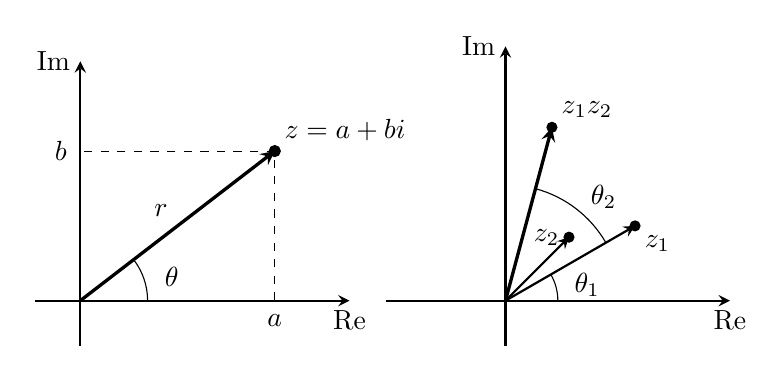
\begin{tikzpicture}[x=0.95cm,y=0.95cm,>=stealth]
 \begin{scope}
  \draw[thick,->] (-0.6,0) -- (3.6,0) node[below] {Re};
  \draw[thick,->] (0,-0.6) -- (0,3.2) node[left] {Im};
  \draw[very thick,->] (0,0) -- (2.6,2.0);
  \draw[dashed] (2.6,0) -- (2.6,2.0) -- (0,2.0);
  \draw[fill] (2.6,2.0) circle (2pt) node[above right] {$z=a+bi$};
  \node[below] at (2.6,-0.05) {$a$};
  \node[left] at (-0.05,2.0) {$b$};
  \draw[thin] (0.9,0) arc[start angle=0,end angle=37.6,radius=0.9];
  \node[right] at (18:1.05) {$\theta$};
  \node[above left] at (1.3,1.0) {$r$};
 \end{scope}
 \begin{scope}[xshift=5.4cm]
  \draw[thick,->] (-1.6,0) -- (3.0,0) node[below] {Re};
  \draw[thick,->] (0,-0.6) -- (0,3.4) node[left] {Im};
  \draw[thick,->] (0,0) -- (1.732,1.0);
  \draw[thick,->] (0,0) -- (0.849,0.849);
  \draw[very thick,->] (0,0) -- (0.621,2.318);
  \draw[fill] (1.732,1.0) circle (1.8pt) node[below right] {$z_{1}$};
  \draw[fill] (0.849,0.849) circle (1.8pt) node[left] {$z_{2}$};
  \draw[fill] (0.621,2.318) circle (1.8pt) node[above right] {$z_{1}z_{2}$};
  \draw[thin] (0.7,0) arc[start angle=0,end angle=30,radius=0.7];
  \node[right] at (15:0.82) {$\theta_{1}$};
  \draw[thin] (30:1.55) arc[start angle=30,end angle=75,radius=1.55];
  \node[right] at (54:1.72) {$\theta_{2}$};
 \end{scope}
\end{tikzpicture}
\end{center}

\begin{idea}[মডুলাস, আর্গুমেন্ট ও পোলার রূপ]
$z = a+bi$-এর মডুলাস $r = |z| = \sqrt{a^{2}+b^{2}}$ হলো মূলবিন্দু থেকে
দূরত্ব, আর আর্গুমেন্ট $\theta = \arg z$ হলো ধনাত্মক বাস্তব অক্ষ থেকে মাপা কোণ।
তখন $a = r\cos\theta$, $b = r\sin\theta$ এবং
\[
  z = r\left( \cos\theta + i\sin\theta \right) .
\]
\end{idea}

এটি ১২ নম্বর অধ্যায়ের polar স্থানাঙ্কেরই আরেক ব্যবহার, তাই সেখানকার
সতর্কতাগুলোও এখানে খাটে: $\theta$ বের করতে কেবল $\tan\theta = b/a$ যথেষ্ট নয়,
কোন চতুর্ভাগে আছে তা দেখে নিতে হবে (১৩ নম্বর অধ্যায়ের $\arctan$-এর
মূল পরিসরের আলোচনাটি মনে করো)। আর $\theta$-তে $2\pi$ যোগ করলে একই সংখ্যা,
তাই আর্গুমেন্ট এককভাবে নির্ধারিত নয় (যদিও আর্গুমেন্টের মুখ্যমান (principal value of argument) $(-\pi,\pi]$ (রেডিয়ানে) বা $(-180^\circ,180^\circ]$ (ডিগ্রীতে) সীমাবদ্ধ।)

এবার এই অনুচ্ছেদের আসল কথা।

\begin{idea}[গুণ মানে ঘূর্ণন ও প্রসারণ]
$z_{1} = r_{1}\left( \cos\theta_{1} + i\sin\theta_{1} \right)$ এবং
$z_{2} = r_{2}\left( \cos\theta_{2} + i\sin\theta_{2} \right)$ হলে
\[
  z_{1}z_{2} = r_{1}r_{2}\left[ \cos(\theta_{1}+\theta_{2})
  + i\sin(\theta_{1}+\theta_{2}) \right] .
\]
অর্থাৎ গুণ করলে মডুলাস গুণ হয় এবং আর্গুমেন্ট যোগ হয়।
\end{idea}

প্রমাণটি ১৩ নম্বর অধ্যায়ের যোগ সূত্র থেকে সরাসরি। খুলে গুণ করি:
\[
  z_{1}z_{2} = r_{1}r_{2}\left[
  \left( \cos\theta_{1}\cos\theta_{2} - \sin\theta_{1}\sin\theta_{2} \right)
  + i\left( \sin\theta_{1}\cos\theta_{2} + \cos\theta_{1}\sin\theta_{2} \right)
  \right] .
\]
বন্ধনী দুটির ভেতরে ঠিক $\cos(\theta_{1}+\theta_{2})$ ও
$\sin(\theta_{1}+\theta_{2})$ বসে আছে।

এটাই সেই আবিষ্কার যা $i$-কে নিছক বীজগণিতের কৌশল থেকে জ্যামিতির যন্ত্রে বদলে
দিয়েছে। বিশেষ ক্ষেত্র: $i$-এর মডুলাস $1$ ও আর্গুমেন্ট $90^{\circ}$, তাই
\emph{$i$ দিয়ে গুণ করা মানে $90^{\circ}$ ঘোরানো}। আর দুবার ঘোরালে
$180^{\circ}$, অর্থাৎ চিহ্ন উল্টে যাওয়া; ঠিক এই কারণেই $i^{2} = -1$।
সংজ্ঞাটা এখন আর খামখেয়ালি লাগছে না।

\begin{example}
$z_{1} = 1+i$ ও $z_{2} = \sqrt{3}+i$-কে পোলার রূপে লিখে গুণফল নির্ণয় করো।
\end{example}

\begin{solbox}
$|z_{1}| = \sqrt{2}$ এবং $z_{1}$ প্রথম চতুর্ভাগে, $\tan\theta = 1$, তাই
$\theta_{1} = 45^{\circ}$।

$|z_{2}| = \sqrt{3+1} = 2$ এবং $\tan\theta = 1/\sqrt{3}$ প্রথম চতুর্ভাগে, তাই
$\theta_{2} = 30^{\circ}$।

সুতরাং
\[
  z_{1}z_{2} = 2\sqrt{2}\left( \cos 75^{\circ} + i\sin 75^{\circ} \right) .
\]
যাচাই সরাসরি গুণ করে: $(1+i)(\sqrt{3}+i) = \sqrt{3} + i + \sqrt{3}i - 1
= (\sqrt{3}-1) + (\sqrt{3}+1)i$। এর মডুলাস
$\sqrt{(\sqrt{3}-1)^{2}+(\sqrt{3}+1)^{2}} = \sqrt{4-2\sqrt{3}+4+2\sqrt{3}}
= \sqrt{8} = 2\sqrt{2}$। মিলে গেল।

পাশাপাশি একটি বোনাস পাওয়া গেল: বাস্তব ও কাল্পনিক অংশ মিলিয়ে
$\cos 75^{\circ} = \dfrac{\sqrt{3}-1}{2\sqrt{2}}$, যা ১৩ নম্বর অধ্যায়ের
যোগ সূত্র দিয়েও বের করা যেত।
\end{solbox}

\prob{2} পোলার রূপে লেখো (মডুলাস ও আর্গুমেন্ট দুটিই দাও)।
\begin{enumerate}
  \item $1+i$
  \item $-\sqrt{3}+i$
  \item $-2i$
\end{enumerate}

\begin{sol}
\begin{enumerate}
  \item $r = \sqrt{2}$, প্রথম চতুর্ভাগ, $\theta = \dfrac{\pi}{4}$।
  \item $r = 2$; বাস্তব অংশ ঋণাত্মক ও কাল্পনিক অংশ ধনাত্মক, তাই দ্বিতীয়
        চতুর্ভাগ। $\tan\theta = -\dfrac{1}{\sqrt{3}}$ দেয় $-30^{\circ}$
        বা $150^{\circ}$; চতুর্ভাগ দেখে $\theta = 150^{\circ} =
        \dfrac{5\pi}{6}$।
  \item $r = 2$, বিন্দুটি ঋণাত্মক কাল্পনিক অক্ষে, তাই
        $\theta = -\dfrac{\pi}{2}$।
\end{enumerate}
দ্বিতীয়টিই দেখাচ্ছে কেন চতুর্ভাগ যাচাই করা বাধ্যতামূলক; ক্যালকুলেটরের
$\arctan$ ভুল উত্তর দিত।
\end{sol}

\prob{2} Argand diagram-এ নিচের প্রতিটি শর্ত কোন বিন্দুসমষ্টি (locus of a point) বোঝায়?
\begin{enumerate}
  \item $|z| = 3$
  \item $|z-2| = 1$
  \item $|z-1| = |z+1|$
\end{enumerate}

\begin{sol}
\begin{enumerate}
  \item মূলবিন্দু থেকে দূরত্ব $3$, অর্থাৎ $3$ ব্যাসার্ধের বৃত্ত।
  \item $|z-2|$ হলো $z$ ও $2$ বিন্দুর দূরত্ব, তাই $(2,0)$ কেন্দ্রবিশিষ্ট
        $1$ ব্যাসার্ধের বৃত্ত।
  \item $1$ ও $-1$ থেকে সমদূরবর্তী বিন্দুগুলো, অর্থাৎ ওই রেখাংশের লম্ব
        সমদ্বিখণ্ডক, যা এখানে কাল্পনিক অক্ষ।
\end{enumerate}
মূল কথা: $|z-w|$ সবসময় দুটি বিন্দুর দূরত্ব। এটি মনে রাখলে এই ধরনের প্রশ্ন
বীজগণিত ছাড়াই ছবি দেখে সমাধান হয়ে যায়।
\end{sol}

\prob{3} $1+i$ দিয়ে গুণ করা মানে জ্যামিতিকভাবে কী, তা বলো। এরপর $0$, $1$,
$1+i$, $i$ শীর্ষবিন্দুবিশিষ্ট বর্গটির প্রতিটি শীর্ষবিন্দুর প্রতিবিম্ব নির্ণয়
করো এবং ফলাফলটি বর্ণনা করো।

\begin{sol}
$|1+i| = \sqrt{2}$ এবং $\arg(1+i) = 45^{\circ}$, তাই $1+i$ দিয়ে গুণ করা মানে
$45^{\circ}$ ঘোরানো এবং $\sqrt{2}$ গুণ প্রসারিত করা।

শীর্ষবিন্দুগুলো:
\[
  0 \mapsto 0, \qquad
  1 \mapsto 1+i, \qquad
  1+i \mapsto (1+i)^{2} = 2i, \qquad
  i \mapsto i(1+i) = -1+i .
\]
প্রতিবিম্বটি আবার একটি বর্গ, শীর্ষবিন্দু $0$, $1+i$, $2i$, $-1+i$। তার বাহুর
দৈর্ঘ্য $\sqrt{2}$, অর্থাৎ মূল বর্গের $\sqrt{2}$ গুণ, আর সে $45^{\circ}$
ঘোরানো। ক্ষেত্রফল $1$ থেকে $2$ হয়েছে, অর্থাৎ $|1+i|^{2}$ গুণ; সদৃশ আকৃতির
ক্ষেত্রফল দৈর্ঘ্যের বর্গের সমানুপাতিক (১১ নম্বর অধ্যায়)।
\end{sol}

\section{অয়লারের সূত্র}

এখন এই অধ্যায়ের কেন্দ্রবিন্দু।

\begin{idea}[অয়লার-এর সূত্র]
\[
  e^{i\theta} = \cos\theta + i\sin\theta .
\]
\end{idea}

১৫ নম্বর অধ্যায়ে তিনটি সিরিজ পাওয়া গিয়েছিল:
\[
  e^{x} = 1 + x + \frac{x^{2}}{2!} + \frac{x^{3}}{3!} + \cdots, \qquad
  \cos x = 1 - \frac{x^{2}}{2!} + \frac{x^{4}}{4!} - \cdots, \qquad
  \sin x = x - \frac{x^{3}}{3!} + \cdots
\]
প্রশ্ন: প্রথমটিতে $x$-এর জায়গায় $i\theta$ বসালে কী হয়?

হিসাবটা করে দেখা যাক। $i$-এর ঘাতগুলো চার ধাপে ঘোরে:
\[
  i^{0}=1, \quad i^{1}=i, \quad i^{2}=-1, \quad i^{3}=-i, \quad i^{4}=1,
  \quad \dots
\]
সিরিজে বসাই:
\[
  e^{i\theta} = 1 + i\theta + \frac{(i\theta)^{2}}{2!}
  + \frac{(i\theta)^{3}}{3!} + \frac{(i\theta)^{4}}{4!} + \cdots
  = 1 + i\theta - \frac{\theta^{2}}{2!} - i\frac{\theta^{3}}{3!}
  + \frac{\theta^{4}}{4!} + \cdots
\]
এবার $i$-যুক্ত পদ আর $i$-বিহীন পদ আলাদা করে সাজাই:
\[
  e^{i\theta} = \left( 1 - \frac{\theta^{2}}{2!} + \frac{\theta^{4}}{4!}
  - \cdots \right)
  + i\left( \theta - \frac{\theta^{3}}{3!} + \frac{\theta^{5}}{5!}
  - \cdots \right) .
\]
প্রথম বন্ধনীটি ঠিক $\cos\theta$-এর সিরিজ, দ্বিতীয়টি $\sin\theta$-এর। সুতরাং
$e^{i\theta} = \cos\theta + i\sin\theta$।

\begin{remark}
উপরের হিসাবটি সুন্দর, কিন্তু সেখানে যা যা ধরে নেওয়া হয়েছে তা গোপন করা
অসাধু হবে। তিনটি জিনিস ধরে নেওয়া হলো।

এক, $e^{z}$ মানে কী তা জটিল $z$-এর জন্য আগে থেকে সংজ্ঞায়িত ছিল না। এখানে
আমরা কার্যত ওই সিরিজটিকেই সংজ্ঞা ধরে নিচ্ছি।

দুই, সিরিজটি জটিল সংখ্যার জন্যও অভিসারী, অর্থাৎ যোগফলটির অর্থ আছে। ১৫ নম্বর
অধ্যায়েই বলা হয়েছিল যে অভিসৃতি এই সিরিজে আলোচিত হবে না; জটিল ক্ষেত্রে
প্রশ্নটা আরও বড়।

তিন, অসীম ধারার পদগুলোকে এভাবে নতুন করে সাজিয়ে দুটি ভাগে ভাগ করা বৈধ। সসীম
যোগফলে এটি নিশ্চয়ই বৈধ, কিন্তু অসীম ধারায় সবসময় নয়; এখানে বৈধ, তবে সেটি
একটি উপপাদ্য।

তিনটিই সত্যি এবং প্রমাণযোগ্য, কিন্তু প্রমাণগুলো এই সিরিজের বাইরে। তাই
বলা ভালো: এটি একটি \emph{যুক্তিসঙ্গত নির্মাণ}, ফাঁকহীন প্রমাণ নয়। তবু এটিকে
সংজ্ঞা বলে চালিয়ে দেওয়ার চেয়ে এভাবে দেখাই ভালো, কারণ তাতে বোঝা যায় সূত্রটি
কোথা থেকে আসছে।
\end{remark}

সূত্রটি হাতে আসায় অনেক কিছু সরল হয়ে যায়।

প্রথমত, পোলার রূপ এখন সংক্ষিপ্ত: $z = re^{i\theta}$। আর তৃতীয় অনুচ্ছেদের
গুণের নিয়মটি এখন নিছক সূচকের নিয়ম:
\[
  r_{1}e^{i\theta_{1}} \cdot r_{2}e^{i\theta_{2}}
  = r_{1}r_{2}\,e^{i(\theta_{1}+\theta_{2})} .
\]
ত্রিকোণমিতির যোগ সূত্র যেখানে লাগত, সেখানে এখন কেবল ঘাত যোগ।

দ্বিতীয়ত, $\theta = \pi$ বসালে $e^{i\pi} = -1$, অর্থাৎ
\[
  e^{i\pi} + 1 = 0 ,
\]
যেখানে $e$, $i$, $\pi$, $1$ ও $0$ একসঙ্গে দাঁড়িয়ে আছে। তাই একে প্রায়ই the most beautiful equation of math বলা হয়!

তৃতীয়ত, De Moivre-এর সূত্র:
\[
  \left( \cos\theta + i\sin\theta \right)^{n}
  = \left( e^{i\theta} \right)^{n} = e^{in\theta}
  = \cos n\theta + i\sin n\theta .
\]

চতুর্থত, $e^{i\theta}$ ও $e^{-i\theta}$ যোগ বা বিয়োগ করে
\[
  \cos\theta = \frac{e^{i\theta}+e^{-i\theta}}{2}, \qquad
  \sin\theta = \frac{e^{i\theta}-e^{-i\theta}}{2i} .
\]
১০ নম্বর অধ্যায়ের $\cosh$ ও $\sinh$-এর সংজ্ঞার সঙ্গে মিলিয়ে দেখো; সেখানে
প্রতিশ্রুতি দেওয়া হয়েছিল যে $\cos^{2}+\sin^{2}=1$ আর
$\cosh^{2}-\sinh^{2}=1$ আসলে একই সম্পর্ক, আর এই দুটি সমীকরণই তার চাবি। বাকিটা
এই অনুচ্ছেদের শেষ সমস্যায়।

\begin{idea}[একের মূল]
$z^{n} = 1$ সমীকরণের $n$টি সমাধান
\[
  z_{k} = e^{2\pi i k/n}, \qquad k = 0, 1, \dots, n-1 .
\]
এরা একক বৃত্তের উপর সমান দূরত্বে বসে থাকে, অর্থাৎ একটি সুষম $n$-ভুজের
শীর্ষবিন্দু।
\end{idea}

কেন: $z = re^{i\theta}$ লিখলে $z^{n} = r^{n}e^{in\theta} = 1$ দাবি করছে
$r^{n} = 1$ (তাই $r = 1$, কারণ $r$ অঋণাত্মক বাস্তব) এবং $n\theta$ হবে
$2\pi$-এর গুণিতক, অর্থাৎ $\theta = \dfrac{2\pi k}{n}$। $k = 0$ থেকে $n-1$
পর্যন্ত আলাদা বিন্দু পাওয়া যায়, তারপর পুনরাবৃত্তি শুরু হয়।

\begin{center}
\begin{tikzpicture}[scale=1.0,>=stealth]
  \draw[thick,->] (-2.4,0) -- (2.6,0) node[below] {Re};
  \draw[thick,->] (0,-2.4) -- (0,2.6) node[left] {Im};
  \draw[thick] (0,0) circle (2);
  \foreach \k in {0,1,2,3,4,5}{
    \pgfmathsetmacro\an{60*\k}
    \draw[dashed] (0,0) -- (\an:2);
    \draw[fill] (\an:2) circle (2.4pt);
  }
  \draw[thick] (0:2) -- (60:2) -- (120:2) -- (180:2) -- (240:2) -- (300:2) -- cycle;
  \node[above right] at (0:2) {$1$};
  \node[right] at (60:2.05) {$\omega$};
  \node[left] at (120:2.05) {$\omega^{2}$};
  \node[left] at (180:2.05) {$\omega^{3}$};
  \node[left] at (240:2.05) {$\omega^{4}$};
  \node[right] at (300:2.05) {$\omega^{5}$};
  \draw[thin] (0.7,0) arc[start angle=0,end angle=60,radius=0.7];
  \node[right] at (30:0.85) {$\tfrac{2\pi}{6}$};
\end{tikzpicture}
\end{center}

ছবিটি $n = 6$-এর। $\omega = e^{2\pi i/6}$ ধরলে বাকি সবাই তার ঘাত, তাই ছয়টি
মূল হলো $1, \omega, \omega^{2}, \dots, \omega^{5}$।

\begin{example}
De Moivre ব্যবহার করে $\cos 2\theta$ ও $\sin 2\theta$ বের করো।
\end{example}

\begin{solbox}
$n = 2$ নিয়ে
\[
  \cos 2\theta + i\sin 2\theta
  = \left( \cos\theta + i\sin\theta \right)^{2}
  = \cos^{2}\theta + 2i\sin\theta\cos\theta + i^{2}\sin^{2}\theta .
\]
$i^{2} = -1$ বসিয়ে বাস্তব ও কাল্পনিক অংশ আলাদা করি:
\[
  \cos 2\theta = \cos^{2}\theta - \sin^{2}\theta, \qquad
  \sin 2\theta = 2\sin\theta\cos\theta .
\]
১৩ নম্বর অধ্যায়ে এই দুটি আলাদা করে বের করতে হয়েছিল; এখানে একটিমাত্র
হিসাবে দুটোই এল, কারণ একটি জটিল সমীকরণ আসলে দুটি বাস্তব সমীকরণ।
\end{solbox}

\prob{2} নির্ণয় করো।
\begin{enumerate}
  \item $e^{i\pi/2}$ ও $e^{-i\pi}$
  \item $2e^{i\pi/3}$-কে $a+bi$ আকারে লেখো
  \item $\left| e^{i\theta} \right|$
\end{enumerate}

\begin{sol}
\begin{enumerate}
  \item $e^{i\pi/2} = \cos 90^{\circ} + i\sin 90^{\circ} = i$;
        $e^{-i\pi} = \cos(-180^{\circ}) + i\sin(-180^{\circ}) = -1$।
  \item $2\left( \cos 60^{\circ} + i\sin 60^{\circ} \right)
        = 2\left( \dfrac{1}{2} + i\dfrac{\sqrt{3}}{2} \right)
        = 1 + i\sqrt{3}$।
  \item $\left| e^{i\theta} \right| = \sqrt{\cos^{2}\theta + \sin^{2}\theta}
        = 1$ সব বাস্তব $\theta$-এর জন্য। অর্থাৎ $e^{i\theta}$ সবসময় একক
        বৃত্তের উপর; সে কেবল দিক বদলায়, দৈর্ঘ্য নয়।
\end{enumerate}
\end{sol}

\prob{3} De Moivre ব্যবহার করে $\cos 3\theta$ ও $\sin 3\theta$ বের করো এবং
১৩ নম্বর অধ্যায়ের ফলের সঙ্গে মেলাও।

\begin{sol}
\[
  \cos 3\theta + i\sin 3\theta
  = \left( \cos\theta + i\sin\theta \right)^{3} .
\]
ডান পাশ খুলি ($c = \cos\theta$, $s = \sin\theta$ লিখে):
\[
  c^{3} + 3c^{2}(is) + 3c(is)^{2} + (is)^{3}
  = c^{3} + 3ic^{2}s - 3cs^{2} - is^{3} .
\]
বাস্তব ও কাল্পনিক অংশ আলাদা করে
\[
  \cos 3\theta = c^{3} - 3cs^{2}, \qquad
  \sin 3\theta = 3c^{2}s - s^{3} .
\]
এবার $s^{2} = 1-c^{2}$ বসালে
\[
  \cos 3\theta = c^{3} - 3c\left( 1-c^{2} \right) = 4\cos^{3}\theta
  - 3\cos\theta ,
\]
যা ১৩ নম্বর অধ্যায়ের ফলের সঙ্গে হুবহু মেলে। একইভাবে $c^{2} = 1-s^{2}$
বসিয়ে $\sin 3\theta = 3\sin\theta - 4\sin^{3}\theta$।

সেখানে যোগ সূত্র দুবার প্রয়োগ করে অর্ধ পৃষ্ঠা লেগেছিল; এখানে একবার ঘন করেই
দুটো ফল একসঙ্গে।
\end{sol}

\prob{3} $z^{3} = 1$ সমীকরণের তিনটি মূল নির্ণয় করো, তাদের Argand diagram-এ
বসাও, এবং প্রমাণ করো যে তাদের যোগফল শূন্য।

\begin{sol}
$z = e^{2\pi ik/3}$, $k = 0,1,2$, অর্থাৎ
\[
  1, \qquad \omega = e^{2\pi i/3} = -\frac{1}{2} + \frac{\sqrt{3}}{2}i,
  \qquad \omega^{2} = e^{4\pi i/3} = -\frac{1}{2} - \frac{\sqrt{3}}{2}i .
\]
তিনটিই একক বৃত্তের উপর, $120^{\circ}$ ব্যবধানে, অর্থাৎ একটি সমবাহু ত্রিভুজের
শীর্ষবিন্দু।

যোগফল: সরাসরি যোগ করলে
$1 - \tfrac{1}{2} - \tfrac{1}{2} = 0$ এবং কাল্পনিক অংশ
$\tfrac{\sqrt{3}}{2} - \tfrac{\sqrt{3}}{2} = 0$, তাই যোগফল শূন্য।

বীজগণিতেও দেখা যায়: $z^{3}-1 = (z-1)\left( z^{2}+z+1 \right)$, তাই $\omega$
ও $\omega^{2}$ হলো $z^{2}+z+1=0$-এর মূল, এবং ৩ নম্বর অধ্যায়ের সম্পর্ক
অনুযায়ী তাদের যোগফল $-1$। এর সঙ্গে $1$ যোগ করলে $0$।

সাধারণভাবে $n \geq 2$ হলে সব $n$-তম মূলের যোগফল শূন্য, কারণ ছবিতে তারা
প্রতিসমভাবে ছড়ানো এবং একে অপরকে কাটাকাটি করে দেয়।
\end{sol}

\prob{4} $\cos\theta$ ও $\sin\theta$-এর সূচকীয় রূপ ব্যবহার করে প্রমাণ করো যে
\[
  \cos(ix) = \cosh x, \qquad \sin(ix) = i\sinh x ,
\]
এবং এখান থেকে দেখাও যে $\cos^{2}+\sin^{2}=1$ অভেদটি $\cosh^{2}x -
\sinh^{2}x = 1$-এ পরিণত হয় (১০ নম্বর অধ্যায়)।

\begin{sol}
$\theta$-এর জায়গায় $ix$ বসাই। প্রথমটিতে:
\[
  \cos(ix) = \frac{e^{i(ix)} + e^{-i(ix)}}{2}
           = \frac{e^{-x} + e^{x}}{2} = \cosh x ,
\]
কারণ $i \cdot i = -1$।

দ্বিতীয়টিতে:
\[
  \sin(ix) = \frac{e^{i(ix)} - e^{-i(ix)}}{2i}
           = \frac{e^{-x} - e^{x}}{2i}
           = \frac{-2\sinh x}{2i} = -\frac{\sinh x}{i} .
\]
এখন $\dfrac{1}{i} = \dfrac{-i}{-i \cdot i} = -i$, সুতরাং
$\sin(ix) = i\sinh x$।

এবার অভেদটিতে বসাই:
\[
  \cos^{2}(ix) + \sin^{2}(ix) = 1
  \;\Longrightarrow\;
  \cosh^{2}x + \left( i\sinh x \right)^{2} = 1
  \;\Longrightarrow\;
  \cosh^{2}x - \sinh^{2}x = 1 .
\]
১০ নম্বর অধ্যায়ে বলা হয়েছিল যে চিহ্নের ওই পার্থক্যটা কাকতালীয় নয়; কারণটা
এখন পরিষ্কার। Hyperbolic ফাংশনগুলো আসলে ত্রিকোণমিতিক ফাংশনই, কেবল কাল্পনিক
কোণে মাপা, আর $i^{2} = -1$ থেকেই যোগ চিহ্নটি বিয়োগ হয়ে যায়।
\end{sol}

\section{প্রয়োগ}

শেষ অনুচ্ছেদে দেখা যাক এই যন্ত্রটি পদার্থবিজ্ঞানে কীভাবে কাজে লাগে। (এই অংশটা একটু জটিল, তাই আপাতত স্কিপ করতে পারো)

\begin{idea}[Phasor]
$A\cos(\omega t + \varphi)$ ধরনের একটি দোলনকে লেখা যায়
\[
  A\cos(\omega t + \varphi)
  = \operatorname{Re}\left[ A e^{i(\omega t + \varphi)} \right]
  = \operatorname{Re}\left[ \left( Ae^{i\varphi} \right)e^{i\omega t} \right] .
\]
এখানে $\tilde{A} = Ae^{i\varphi}$ জটিল সংখ্যাটিকে বলে phasor; সে একই সঙ্গে
বিস্তার ($|\tilde{A}| = A$) ও আদি দশা ($\arg\tilde{A} = \varphi$) বহন করে।
\end{idea}

কেন এটি কাজের? কারণ একই কম্পাঙ্কের দুটি দোলন যোগ করা মানে তাদের phasor দুটি
যোগ করা, আর জটিল সংখ্যা যোগ করা মানে কেবল বাস্তব ও কাল্পনিক অংশ যোগ করা।
$e^{i\omega t}$ গুণনীয়কটি দুটোতেই সাধারণ, তাই বাইরে বেরিয়ে আসে:
\[
  \operatorname{Re}\left[ \tilde{A}_{1}e^{i\omega t} \right]
  + \operatorname{Re}\left[ \tilde{A}_{2}e^{i\omega t} \right]
  = \operatorname{Re}\left[ \left( \tilde{A}_{1}+\tilde{A}_{2} \right)
    e^{i\omega t} \right] .
\]
১৩ নম্বর অধ্যায়ে $a\cos\theta + b\sin\theta$-কে একটি cosine-এ আনতে
আলাদা কৌশল লেগেছিল; phasor দিয়ে সেটি নিছক দুটি সংখ্যা যোগ।

\begin{center}
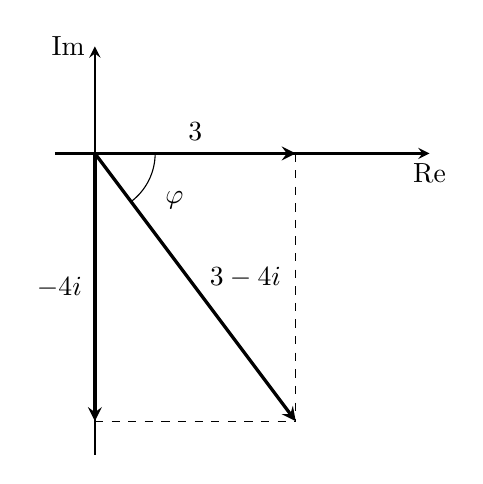
\begin{tikzpicture}[x=0.85cm,y=0.85cm,>=stealth]
  \draw[thick,->] (-0.6,0) -- (5.0,0) node[below] {Re};
  \draw[thick,->] (0,-4.5) -- (0,1.6) node[left] {Im};
  \draw[very thick,->] (0,0) -- (3,0);
  \draw[very thick,->] (0,0) -- (0,-4) ;
  \draw[dashed] (3,0) -- (3,-4);
  \draw[dashed] (0,-4) -- (3,-4);
  \draw[very thick,->] (0,0) -- (3,-4);
  \node[above] at (1.5,0.05) {$3$};
  \node[left] at (-0.05,-2.0) {$-4i$};
  \node at (2.25,-1.85) {$3-4i$};
  \draw[thin] (0.9,0) arc[start angle=0,end angle=-53.13,radius=0.9];
  \node[below right] at (-25:1.0) {$\varphi$};
\end{tikzpicture}
\end{center}

\begin{remark}
Phasor-এর দ্বিতীয় বড় সুবিধা derivative-এ। $e^{i\omega t}$-এর সময়ের সাপেক্ষে
derivative নিলে পাওয়া যায় $i\omega e^{i\omega t}$, অর্থাৎ derivative নেওয়া
মানে কেবল $i\omega$ দিয়ে গুণ করা। ফলে দোলন-সংক্রান্ত differential equation
বীজগণিতের সমীকরণে নেমে আসে। এই কৌশলটিই ১৯ নম্বর অধ্যায়ে ব্যবহার করা হবে,
আর AC বর্তনীর impedance-এর গোটা ধারণাটি এর উপরেই দাঁড়ানো।
\end{remark}

\begin{example}
Phasor ব্যবহার করে $2\cos\omega t + 2\sqrt{3}\sin\omega t$-কে একটিমাত্র
cosine আকারে লেখো।
\end{example}

\begin{solbox}
প্রথমে দ্বিতীয় পদটিকে cosine-এ বদলাই: $\sin\theta =
\cos\left( \theta - 90^{\circ} \right)$, তাই দ্বিতীয় দোলনের দশা
$-90^{\circ}$।

Phasor দুটি:
\[
  \tilde{A}_{1} = 2, \qquad
  \tilde{A}_{2} = 2\sqrt{3}\,e^{-i\pi/2} = -2\sqrt{3}\,i .
\]
যোগ করে $\tilde{A} = 2 - 2\sqrt{3}\,i$, যার মডুলাস
\[
  |\tilde{A}| = \sqrt{4 + 12} = 4
\]
এবং আর্গুমেন্ট: বিন্দুটি চতুর্থ চতুর্ভাগে, $\tan\varphi = -\sqrt{3}$, তাই
$\varphi = -60^{\circ}$। সুতরাং
\[
  2\cos\omega t + 2\sqrt{3}\sin\omega t = 4\cos\left( \omega t
  - 60^{\circ} \right) .
\]
যাচাই: ডান পাশ খুললে $4\left( \cos\omega t\cos 60^{\circ}
+ \sin\omega t\sin 60^{\circ} \right) = 2\cos\omega t
+ 2\sqrt{3}\sin\omega t$। মিলে গেল।
\end{solbox}

\prob{3} Phasor ব্যবহার করে $3\cos\omega t + 4\sin\omega t$-কে
$R\cos(\omega t - \varphi)$ আকারে লেখো, এবং ১৩ নম্বর অধ্যায়ে একই রাশির
জন্য পাওয়া উত্তরের সঙ্গে মেলাও।

\begin{sol}
$4\sin\omega t = 4\cos\left( \omega t - 90^{\circ} \right)$, তাই phasor দুটি
$3$ ও $4e^{-i\pi/2} = -4i$। যোগফল
\[
  \tilde{A} = 3 - 4i .
\]
মডুলাস $\sqrt{9+16} = 5$; আর্গুমেন্ট চতুর্থ চতুর্ভাগে,
$\tan\varphi = -\tfrac{4}{3}$, তাই $\varphi \approx -53.13^{\circ}$। সুতরাং
\[
  3\cos\omega t + 4\sin\omega t = 5\cos\left( \omega t - 53.13^{\circ}
  \right) .
\]
১৩ নম্বর অধ্যায়ে $3\cos\theta + 4\sin\theta = 5\cos(\theta -
53.13^{\circ})$ পাওয়া গিয়েছিল, হুবহু এক। পার্থক্য কেবল পথে: সেখানে
$R = \sqrt{a^{2}+b^{2}}$ ও $\tan\alpha = b/a$ মনে রাখতে হয়েছিল, এখানে দুটি
জটিল সংখ্যা যোগ করাই যথেষ্ট, আর মডুলাস-আর্গুমেন্ট এমনিতেই ওই দুটি সূত্র।
\end{sol}

\prob{4} সমান বিস্তার $A$ ও সমান কম্পাঙ্কের দুটি তরঙ্গের দশার পার্থক্য
$\delta$।
\begin{enumerate}
  \item Phasor ব্যবহার করে দেখাও যে লব্ধির বিস্তার
        $2A\left| \cos\dfrac{\delta}{2} \right|$।
  \item কোন কোন $\delta$-তে লব্ধি শূন্য, এবং কোনগুলোতে সর্বোচ্চ?
\end{enumerate}

\begin{sol}
\begin{enumerate}
  \item Phasor দুটি $A$ ও $Ae^{i\delta}$, তাই যোগফল
        \[
          \tilde{A} = A\left( 1 + e^{i\delta} \right) .
        \]
        কৌশল: বন্ধনী থেকে $e^{i\delta/2}$ বের করে আনি:
        \[
          1 + e^{i\delta} = e^{i\delta/2}\left( e^{-i\delta/2}
          + e^{i\delta/2} \right) = e^{i\delta/2} \cdot 2\cos\frac{\delta}{2} ,
        \]
        যেখানে শেষ ধাপে চতুর্থ অনুচ্ছেদের $\cos$-এর সূচকীয় রূপ ব্যবহার করা
        হয়েছে। সুতরাং
        \[
          \tilde{A} = 2A\cos\frac{\delta}{2}\;e^{i\delta/2} ,
        \]
        অর্থাৎ বিস্তার $2A\left| \cos\dfrac{\delta}{2} \right|$ এবং লব্ধির
        দশা ঠিক দুটির মাঝামাঝি, $\dfrac{\delta}{2}$।
  \item শূন্য হয় যখন $\cos\dfrac{\delta}{2} = 0$, অর্থাৎ
        $\dfrac{\delta}{2} = \dfrac{\pi}{2} + k\pi$, অর্থাৎ
        $\delta = \pi, 3\pi, 5\pi, \dots$; এটিই ধ্বংসাত্মক ব্যতিচার।

        সর্বোচ্চ ($=2A$) হয় যখন $\cos\dfrac{\delta}{2} = \pm 1$, অর্থাৎ
        $\delta = 0, 2\pi, 4\pi, \dots$; এটিই গঠনমূলক ব্যতিচার।
\end{enumerate}
আলোর ব্যতিচারে পথপার্থক্য $\Delta$ থেকে $\delta = \dfrac{2\pi\Delta}{\lambda}$
আসে, তাই উপরের শর্তগুলো চেনা রূপ নেয়: $\Delta$ তরঙ্গদৈর্ঘ্যের পূর্ণসংখ্যক
গুণিতক হলে উজ্জ্বল, অর্ধ-বিজোড় গুণিতক হলে অন্ধকার।
\end{sol}

\end{document}
